\documentclass[tikz]{standalone}

\usepackage{amsmath}
\usepackage{circuitikz}

\usetikzlibrary{positioning}

\begin{document}
	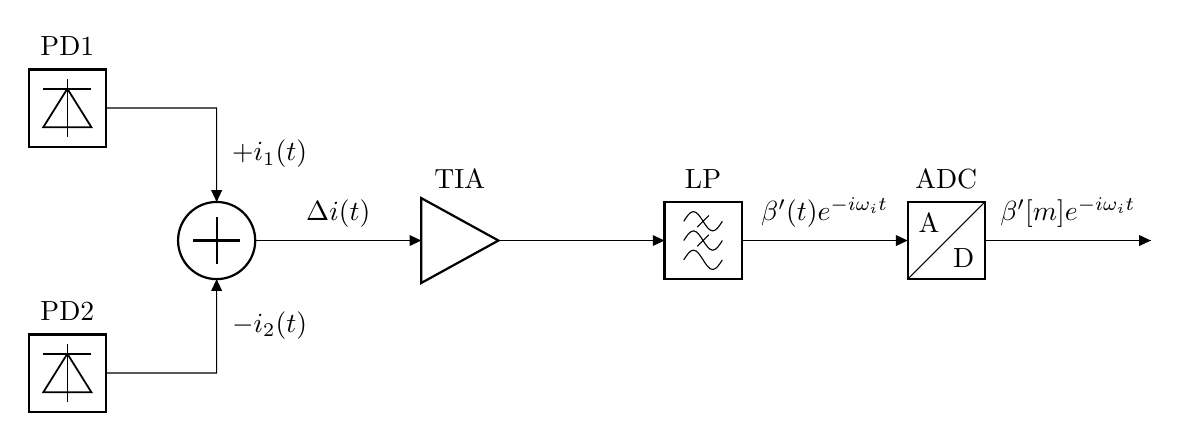
\begin{tikzpicture}[
		node distance=6em,
	]
		\coordinate (in) at (0,0);
		\node [adder, right=of in] (adder) {};
		\node [detectorshape, above left=2em and 4em of adder, label=right:PD1, rotate=90, anchor=west] (pd1) {};
		\node [detectorshape, below left=2em and 4em of adder, label=right:PD2, rotate=90, anchor=east] (pd2) {};
		\node [ampshape, right=of adder, label=TIA] (tia) {};
		\node [lowpassshape, right=of tia, label=LP] (lp) {};
		\node [adcshape, right=of lp, label=ADC] (adc) {};
		\coordinate [right=of adc] (out);
		
		\draw (pd1.south) -- (pd1.south-|adder.north) to[short, l=$+i_1(t)$] (adder.north) node[inputarrow, rotate=-90]{};
		\draw (pd2.south) -- (pd2.south-|adder.south) to[short, l_=$-i_2(t)$] (adder.south) node[inputarrow, rotate=90]{};
		\draw (adder.east) to[short, l={$\Delta i(t)$}] (tia.west) node[inputarrow]{};
		\draw (tia.east) -- (lp.west) node[inputarrow]{};
		\draw (lp.east) to[short, l=$\beta^\prime(t)e^{-i\omega_it}$] (adc.west) node[inputarrow]{};
		\draw (adc.east) to[short, l={$\beta^\prime[m]e^{-i\omega_it}$}] (out) node[inputarrow]{};
	\end{tikzpicture}
\end{document}
